

\chapter{Week 13 -- Overcurrent Protection For A Modular System}

\section{Abstract}
This report presents results of tuning a high-level supervisory algorithm that calculates a system-level current limit respecting the current limitation of individual modules connected in parallel. Different initial conditions of individual modules are assumed for generality. Two solutions are considered -- a feedforward approach based on the closed-form expression for current upper and lower bound using the provided voltage, current and internal resistance of each module, and a feedback solution using a modified PID controller regulating the module current towards the module current limit. 


\section{Problem statement}



\begin{figure}[b]
\centering
\begin{minipage}{0.49\textwidth}
    \centering
    \includegraphics[width=\linewidth]{figures/13/ff-R.pdf}
    \caption{Estimates of the module internal impedance available to the algorithm.}
    \label{fig:13-R}
\end{minipage}
\hfill
\begin{minipage}{0.49\textwidth}
    \centering
    \includegraphics[width=\linewidth]{figures/13/ff-SoC.pdf}
    \caption{Module state of charge (SoC) during the simulation.}
    \label{fig:13-SoC}
\end{minipage}
\end{figure}

\begin{figure}[]
\centering
\begin{minipage}{0.49\textwidth}
    \centering
    \includegraphics[width=\linewidth]{figures/13/fb-IE.pdf}
    \caption{Equalizing current flowing from module 1 to module 2.}
    \label{fig:13-IE}
\end{minipage}
\hfill
\begin{minipage}{0.49\textwidth}
    \centering
    \includegraphics[width=\linewidth]{figures/13/ff-U.pdf}
    \caption{Module terminal voltages.}
    \label{fig:13-U}
\end{minipage}
\end{figure}

The given Simulink model contains a model of two battery modules connected in parallel, each consisting of a 1RC equivalent circuit model (ECM). Each module is given a different initial SoC, as shown in fig. \ref{fig:13-SoC} and also different parameters of the ECM, such as internal impedance $R_0$ shown in Fig. \ref{fig:13-R}. This alone results in some current asymmetry between both modules due to the flow of an equalizing current shown in Fig. \ref{fig:13-IE}. Since both modules are connected in parallel, their terminal voltages must be equal by definition. This is verified in Fig. \ref{fig:13-U}, showing maximal voltage deviation in the order of $10^{-4}$ V.

Each module is given a current limit of 50 A for both charging and discharging. During the experiment, some connected system (e.g. the motor controller of an EV) requests current for vehicle propulsion and the battery system must restrict the current flow to a safe system-wide limit such that neither of the modules is overloaded.

The task is complicated by the measurement noise that is gradually added to the quantities provided to the control algorithm. Furthermore, the estimate of module impedance is subject to significant disturbance, resulting in large variations of the estimate of $R_0$ available for the current limit calculation, as shown in Fig. \ref{fig:13-R}.

\section{Analytical solution}

The first solution utilized an algorithm based on a closed-form expression for the current limit. Measured module voltages, currents and impedances are used to calculate the equalizing current $I_E$. Then, considering the current divider formed by impedances $R_{0,1}$ and $R_{0,2}$, a set of inequalities for the upper bounds of the system current is constructed. The lowest bound is then used to prevent exceeding the current limit fo any module.

Results obtained by this algorithm are shown in Fig. \ref{fig:13-ff-system} and \ref{fig:13-ff-subsystem}. The algorithm has the potential to work very well when provided with correct information (as shown for $t<150$ s), where the current through the first module is saturated perfectly at the module current limit. Nevertheless, as soon as the estimate of $R_0$ becomes noisy or completely wrong, the inherently open-loop solution can't optimally deliver the requested current. This is illustrated for $t > 450$ s, when the system-wide current limit abruptly decreases due to the error of resistance estimates from Fig. \ref{fig:13-R}.

Due to this inherent limitation, the algorithm was not even completely implemented and yielded incorrect results when approaching the negative lower bound. The alternative feedback solution achieved much better performance; hence, it was not worthwhile to attempt to fix the feedforward algorithm. 

\begin{figure}
\centering
\begin{minipage}{0.49\textwidth}
    \centering
    \includegraphics[width=\linewidth]{figures/13/ff-system.pdf}
    \caption{System currents using the feedforward control algorithm.}
    \label{fig:13-ff-system}
\end{minipage}
\hfill
\begin{minipage}{0.49\textwidth}
    \centering
    \includegraphics[width=\linewidth]{figures/13/ff-subsystem.pdf}
    \caption{Subsystem currents using the feedforward algorithm.}
    \label{fig:13-ff-subsystem}
\end{minipage}
\end{figure}

\section{Feedback algorithm}

The feedback algorithm uses a modified PID controller to determine the system-wide current limit. First, since the module current limit is symmetric for charging and discharging, the maximum of absolute values of both module currents is taken to simplify calculations by considering only the positive branch. This maximal current is subtracted from the module current limit to get an error that is fed to the discrete-time PID controller with filtered derivative. The output of the PID controller was saturated at twice the module current limit -- that is the optimistic solution in case both modules are balanced and there is no equalizing current.

To further improve the behavior of the PID controller, the following trick was introduced -- the error is scaled down by a factor of 1000 when it is positive. This way, the current limit is quickly adjusted down to prevent stress to battery modules, while the growth of the current limit is very slow to ensure smooth waveform.

The performance of this algorithm is shown in Fig. \ref{fig:13-fb-system} and \ref{fig:13-fb-subsystem}. It is clear that the algorithm asymptotically delivers the maximal possible current whilst achieving overshoots of both low height as well as area, as shown in Fig. \ref{fig:13-fb-subsystem-detail} and \ref{fig:13-fb-subsystem-detail2}. Typical overshoot is less than 8 A in height and lasts for less than 400 ms.

\begin{figure}
\centering
\begin{minipage}{0.49\textwidth}
    \centering
    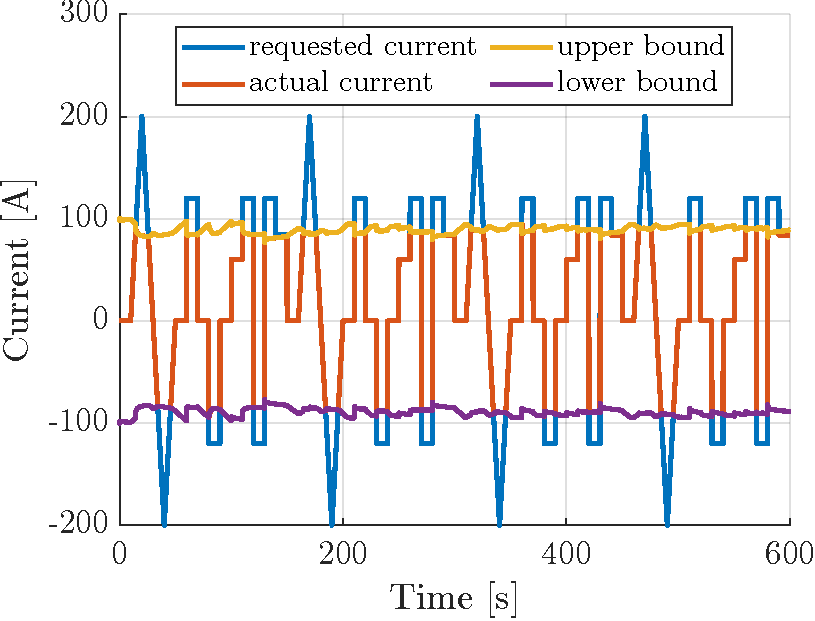
\includegraphics[width=\linewidth]{figures/13/fb-system.pdf}
    \caption{System current using the feedback control algorithm.}
    \label{fig:13-fb-system}
\end{minipage}
\hfill
\begin{minipage}{0.49\textwidth}
    \centering
    \includegraphics[width=\linewidth]{figures/13/fb-subsystem.pdf}
    \caption{Subsystem currents using the feedback algorithm.}
    \label{fig:13-fb-subsystem}
\end{minipage}
\end{figure}


\begin{figure}
\centering
\begin{minipage}{0.49\textwidth}
    \centering
    \includegraphics[width=\linewidth]{figures/13/fb-subsystem-detail.pdf}
    \caption{Overshoots of the module current limit}
    \label{fig:13-fb-subsystem-detail}
\end{minipage}
\hfill
\begin{minipage}{0.49\textwidth}
    \centering
    \includegraphics[width=\linewidth]{figures/13/fb-subsystem-detail2.pdf}
    \caption{Detail of one particular overshoot of the OCP limit.}
    \label{fig:13-fb-subsystem-detail2}
\end{minipage}
\end{figure}

Fig. \ref{fig:13-fb-system-detail} illustrates that a step of the requested system current from 0 to 120 A results in a decrease of the current limit from 94 A to 86 A. This was the worst case (greatest in magnitude) sudden change observed in the simulation outputs.

\begin{figure}
    \centering
    \includegraphics[width=0.5\linewidth]{figures/13/fb-system-detail.pdf}
    \caption{Response of the system-wide current limit to a step of requested current.}
    \label{fig:13-fb-system-detail}
\end{figure}

\section{Conclusions}

The achieved performance could be further improved by giving the algorithm access to the requested current. That way, the algorithm could identify time instants when the flow of current is saturated and only then activate the integrator to slowly increase the system-wide current limit. Without this information the algorithm has to slowly increase the current limit at all times in order to be able to quickly deliver the maximal possible current.

